\chapter{Préparation à l'Entretien Oral}

\begin{tcolorbox}[colback=red!4!white,colframe=red!60!black,title=\textbf{Ce qui est confirmé et ce qui ne l'est pas}]
La convocation et l'avis officiel confirment un \textbf{entretien oral} pour les candidats admissibles à l'écrit, sans en préciser la date, la durée exacte ni la composition du jury. D'après le format observé pour la catégorie \og cadres Bac+5 \fg{} des sociétés régionales multiservices, il s'agit généralement d'un entretien de \textbf{15 à 30 minutes} devant un jury mêlant responsables RH et responsables techniques (souvent la Direction des Systèmes d'Information et la Direction Centrale). Ce chapitre prépare cette hypothèse la plus probable, à ajuster dès que la convocation à l'oral précisera le format réel.
\end{tcolorbox}

\section{Les Cinq Piliers de l'Entretien}
\begin{enumerate}
    \item \textbf{Motivation et connaissance de l'entreprise :} pourquoi la SRM Souss-Massa, pourquoi le secteur de l'eau/électricité, pourquoi ce moment (délai court après convocation).
    \item \textbf{Compétences techniques Génie Informatique :} capacité à expliquer simplement un projet, une architecture ou un choix technique déjà réalisé.
    \item \textbf{Posture de service public :} comprendre que le SI sert la continuité d'un service essentiel (eau, électricité) pour 3 millions d'habitants, pas seulement une performance technique abstraite.
    \item \textbf{Questions RH classiques :} parcours, forces et faiblesses, gestion du stress et des délais, travail en équipe.
    \item \textbf{Actualité et enjeux du secteur :} stress hydrique, dessalement, transformation digitale des services publics régionaux.
\end{enumerate}

\IfFileExists{images/img_015_oral_pyramide_5_piliers.png}{%
\begin{figure}[H]
    \centering
    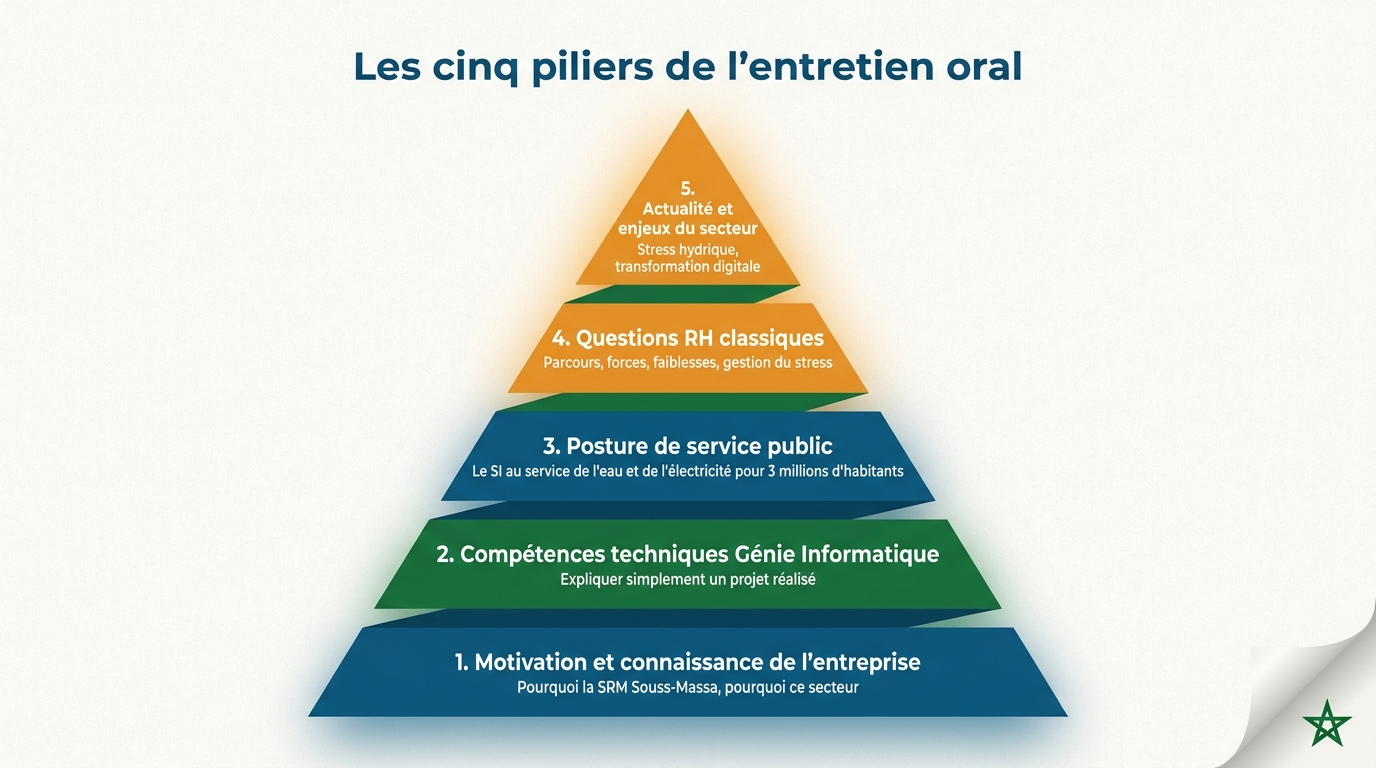
\includegraphics[width=0.85\textwidth]{images/img_015_oral_pyramide_5_piliers.png}
    \caption{Les cinq piliers de l'entretien oral, du plus fondamental (base) au plus spécifique (sommet)}
\end{figure}}{}

\section{Questions Probables et Réponses Modèles Courtes}

{\small
\begin{longtable}{|>{\raggedright\arraybackslash\hspace{0pt}}p{5.2cm}|>{\raggedright\arraybackslash\hspace{0pt}}p{8.8cm}|}
\hline
\rowcolor{gray!20} \textbf{Question probable} & \textbf{Piste de réponse courte} \\ \hline
\endfirsthead
\hline
\rowcolor{gray!20} \textbf{Question probable} & \textbf{Piste de réponse courte} \\ \hline
\endhead

Présentez-vous en deux minutes. & Parcours académique (diplôme, spécialité GI), une ou deux expériences ou projets marquants, puis un lien direct vers le poste visé (pourquoi ce profil correspond à un poste de Direction Centrale). \\ \hline

Pourquoi voulez-vous rejoindre la SRM Souss-Massa ? & Combiner motivation concrète (service public essentiel, région d'origine ou d'attache éventuelle, ampleur du projet de modernisation 2025-2029) et motivation technique (systèmes d'information critiques, SIG, télérelève à fort enjeu). \\ \hline

Qu'apporteriez-vous en tant qu'ingénieur Génie Informatique à une société d'eau et d'électricité ? & Fiabilité et sécurité des systèmes d'information de gestion clientèle, exploitation de la donnée pour optimiser un réseau en stress hydrique, contribution à la cybersécurité d'infrastructures sensibles. \\ \hline

Décrivez un projet technique dont vous êtes fier. & Utiliser la méthode STAR (Situation, Tâche, Action, Résultat) : contexte bref, votre rôle précis, ce que vous avez concrètement fait, le résultat mesurable. \\ \hline

Comment réagiriez-vous face à un incident de cybersécurité sur un système critique ? & Détection et confinement immédiat, remontée hiérarchique selon une procédure définie, analyse post-incident, conformité avec la loi 05-20 ; insister sur la rapidité et la communication claire. \\ \hline

Que savez-vous de la loi 83-21 et de la création de la SRM Souss-Massa ? & Réciter les repères du chapitre 2 : adoption 12 juin 2023, dahir du 12 juillet 2023, activité depuis le 15 octobre 2024, succession de la RAMSA, périmètre et missions. \\ \hline

Quelles sont vos principales qualités et vos axes d'amélioration ? & Une qualité alignée avec le poste (rigueur, capacité d'analyse) illustrée d'un exemple bref ; un axe d'amélioration réel mais non disqualifiant, avec une action concrète déjà engagée pour le corriger. \\ \hline

Comment gérez-vous les délais serrés et la pression ? & Exemple concret de priorisation (méthode, outil, communication proactive) plutôt qu'une réponse abstraite. \\ \hline

Où vous voyez-vous dans cinq ans ? & Montrer une trajectoire cohérente avec une évolution au sein d'une entreprise publique régionale (expertise technique approfondie ou évolution vers l'encadrement), sans sur-promettre. \\ \hline

Avez-vous des questions à nous poser ? & Toujours préparer une ou deux questions sur l'organisation de la DSI, les projets en cours (SIG, télérelève) ou les perspectives d'évolution --- ne jamais répondre \og non \fg{}. \\ \hline

\end{longtable}
}

\section{La Méthode STAR pour les Questions Comportementales}
\begin{enumerate}
    \item \textbf{Situation :} contexte en une ou deux phrases (où, quand, quel projet).
    \item \textbf{Tâche :} ce qui vous était précisément demandé ou ce que vous avez décidé de faire.
    \item \textbf{Action :} ce que VOUS avez fait concrètement (éviter le \og nous \fg{} permanent qui dilue votre contribution).
    \item \textbf{Résultat :} un résultat si possible chiffré ou vérifiable, et ce que vous en avez retenu.
\end{enumerate}

\section{Questions Techniques par Spécialité}
Le poste couvre six spécialités (GI/SI/RT/IA \& DATA/GL/CYBER). Les questions techniques générales de Génie Informatique du tableau précédent restent valables pour tous ; voici en complément une question probable par spécialité, à adapter à votre profil précis si vous couvrez plusieurs domaines.

{\small
\begin{longtable}{|>{\raggedright\arraybackslash\hspace{0pt}}p{2.6cm}|>{\raggedright\arraybackslash\hspace{0pt}}p{5.0cm}|>{\raggedright\arraybackslash\hspace{0pt}}p{6.4cm}|}
\hline
\rowcolor{gray!20} \textbf{Spécialité} & \textbf{Question probable} & \textbf{Piste de réponse} \\ \hline
\endfirsthead
\hline
\rowcolor{gray!20} \textbf{Spécialité} & \textbf{Question probable} & \textbf{Piste de réponse} \\ \hline
\endhead

SI (Systèmes d'Information) & Comment intégreriez-vous les systèmes hérités de la RAMSA dans un SI unifié pour la SRM ? & Cartographier l'existant, prioriser les données critiques (facturation, abonnés), migrer progressivement plutôt qu'en une fois, garantir la continuité de service pendant la transition. \\ \hline

RT (Réseaux et Télécommunications) & Comment concevriez-vous la connectivité de compteurs intelligents répartis sur un territoire aussi vaste que la région Souss-Massa ? & Combiner plusieurs technologies selon la zone (réseau bas débit longue portée pour les zones rurales, 4G/fibre pour les zones urbaines), avec redondance et supervision centralisée. \\ \hline

IA \& DATA & Comment l'exploitation de données pourrait-elle aider la SRM à anticiper les fuites sur le réseau d'eau ? & Analyser les écarts entre volumes produits et facturés, croiser avec les données de télérelève et l'âge des canalisations, pour prioriser les interventions préventives plutôt que curatives. \\ \hline

GL (Génie Logiciel) & Comment garantiriez-vous la qualité d'une application de facturation critique ? & Tests automatisés à chaque étape (unitaires, intégration), revue de code systématique, déploiements progressifs, plan de retour en arrière en cas d'anomalie. \\ \hline

CYBER (Cybersécurité) & Quelles mesures prioriseriez-vous pour protéger le système de supervision technique (SCADA) d'une société d'eau et d'électricité ? & Isolation réseau des systèmes industriels (segmentation), authentification forte, journalisation et supervision continue (SIEM/SOC), conformité à la loi 05-20. \\ \hline

\end{longtable}
}

\section{Cinq Mises en Situation pour s'Entraîner}
Pour chaque mise en situation : une question type, une réponse recommandée, pourquoi elle fonctionne, et une erreur à éviter. À travailler à voix haute, sans jamais apprendre un texte par cœur --- seule la structure doit être mémorisée, les mots doivent rester naturels.

\begin{tcolorbox}[colback=blue!4!white,colframe=blue!40!black,title=\textbf{Simulation 1 --- RH}]
\textbf{Question :} \og Pourquoi devrions-nous vous choisir plutôt qu'un autre candidat ? \fg{}\\
\textbf{Réponse recommandée :} Relier un ou deux atouts concrets (une compétence rare, une expérience directement transférable) à un besoin réel du poste, sans dénigrer les autres candidats.\\
\textbf{Pourquoi ça fonctionne :} Le jury retient l'adéquation précise au poste, pas une liste de qualités génériques.\\
\textbf{Erreur à éviter :} Répondre par une liste de qualités vagues (\og je suis sérieux, motivé \fg{}) sans preuve ni exemple.
\end{tcolorbox}

\begin{tcolorbox}[colback=blue!4!white,colframe=blue!40!black,title=\textbf{Simulation 2 --- Technique}]
\textbf{Question :} \og Expliquez-moi la différence entre une base de données relationnelle et une base NoSQL, avec un exemple d'usage pour notre secteur. \fg{}\\
\textbf{Réponse recommandée :} Définition simple des deux (voir chapitre 3), puis exemple concret : relationnelle pour la facturation (transactions fiables), NoSQL pour de gros volumes de mesures de télérelève horodatées.\\
\textbf{Pourquoi ça fonctionne :} Montre une compréhension technique ET sa mise en contexte dans le métier de l'entreprise, pas juste une définition apprise par cœur.\\
\textbf{Erreur à éviter :} Réciter une définition technique sans jamais la relier au métier de la SRM.
\end{tcolorbox}

\begin{tcolorbox}[colback=blue!4!white,colframe=blue!40!black,title=\textbf{Simulation 3 --- Entreprise SRM}]
\textbf{Question :} \og Que savez-vous des grands projets actuels de la SRM Souss-Massa ? \fg{}\\
\textbf{Réponse recommandée :} Citer deux ou trois faits précis et datés du chapitre 2 (méga-projet Tiznit--Chtouka annoncé le 27 août 2026, station de dessalement de Chtouka-Aït Baha, plan quinquennal 2025-2029), puis relier brièvement au rôle des systèmes d'information dans leur pilotage.\\
\textbf{Pourquoi ça fonctionne :} Prouve une préparation sérieuse et une compréhension du lien entre votre métier et la stratégie de l'entreprise.\\
\textbf{Erreur à éviter :} Rester vague (\og je sais qu'ils font des projets d'eau \fg{}) sans aucun fait précis.
\end{tcolorbox}

\begin{tcolorbox}[colback=blue!4!white,colframe=blue!40!black,title=\textbf{Simulation 4 --- Mise en Situation Professionnelle}]
\textbf{Question :} \og Un incident bloque le système de facturation un vendredi soir, avec un impact direct sur les abonnés. Que faites-vous ? \fg{}\\
\textbf{Réponse recommandée :} Décrire une démarche structurée : évaluer l'impact et la criticité, contenir le problème (isoler si nécessaire), communiquer immédiatement aux responsables selon une procédure d'escalade, corriger, puis documenter l'incident pour éviter sa répétition.\\
\textbf{Pourquoi ça fonctionne :} Montre une capacité à structurer sa pensée sous pression plutôt que de paniquer ou d'improviser.\\
\textbf{Erreur à éviter :} Répondre uniquement par une solution technique sans mentionner la communication vers la hiérarchie et les utilisateurs impactés.
\end{tcolorbox}

\begin{tcolorbox}[colback=blue!4!white,colframe=blue!40!black,title=\textbf{Simulation 5 --- Question Déstabilisante}]
\textbf{Question :} \og Vous n'avez jamais travaillé dans le secteur de l'eau ou de l'électricité. Pourquoi devrions-nous vous faire confiance ? \fg{}\\
\textbf{Réponse recommandée :} Reconnaître le fait calmement sans se justifier excessivement, puis mettre en avant ce qui est transférable (les fondamentaux des systèmes d'information et de la cybersécurité sont les mêmes quel que soit le secteur) et une preuve de capacité d'apprentissage rapide.\\
\textbf{Pourquoi ça fonctionne :} Le jury teste la gestion du stress et l'honnêteté autant que la réponse elle-même ; une réponse calme et structurée rassure davantage qu'une justification défensive.\\
\textbf{Erreur à éviter :} Se braquer, nier le manque d'expérience sectorielle, ou au contraire s'excuser de façon excessive.
\end{tcolorbox}

\section{Erreurs qui Font Perdre des Points à l'Oral}
\begin{itemize}
    \item Réciter le CV sans le relier au poste visé.
    \item Ne rien savoir de l'entreprise au-delà de son nom (dates, missions, chiffres clés du chapitre 2 à maîtriser).
    \item Répondre uniquement en termes techniques abstraits sans jamais relier au service rendu aux usagers.
    \item Critiquer un ancien employeur ou une expérience précédente de façon négative.
    \item Ne poser aucune question au jury en fin d'entretien.
    \item Improviser sur les faits et chiffres de l'entreprise plutôt que de les avoir mémorisés avec précision.
\end{itemize}

\section{Checklist du Jour de l'Entretien}
\begin{enumerate}
    \item Relire le résumé exécutif et le chapitre 2 (entreprise) juste avant l'entretien.
    \item Préparer une présentation de deux minutes chronométrée et répétée à voix haute.
    \item Préparer deux exemples de projets techniques détaillables selon la méthode STAR.
    \item Préparer une ou deux questions à poser au jury.
    \item Tenue professionnelle sobre, CIN et convocation à l'oral en main, arrivée en avance.
\end{enumerate}
